\chapter{Platformy low-code/no-code}\label{cha:low}
Low-Code oraz no-code to nowe podejście skupiające się na tworzeniu oprogramowania bez konieczności znajomości języka programowania.\ Celem tych działań jest umożliwienie osobom nietechnicznym, które nie są programistami, na łatwe i szybkie tworzenie aplikacji biznesowych.\ Pozwoli to odpowiedzieć na rosnące zapotrzebowanie na wytwarzanie oprogramowania, rozwiązań biznesowych, przy brakującej liczbie programistów, która mogłaby sprostać potrzebom rynku.
\\ \\
Podejście low-code/no-code jest dość nowym rozwiązaniem.\ Początki tego podejścia można zauważyć w narzędziach umożliwiających samodzielne tworzenie stron internetowych np. \textit{Wordpress}, \textit{Joomla} czy \textit{Wix}.\ Dzięki tym rozwiązaniom, stronę można utworzyć w łatwy sposób, za pomocą tzw. kafelków.\ Kafelki to komponenty, które pozwalają na umieszczenie tekstu, grafiki, wideo czy innych elementów na stronie~\cite{Wordpress2023,Joomla2023,Wix2023}.\ Na \refsource{rysunkach}{fig:pa-plat},~\textbf{\ref{fig:wp-plat}} przedstawiono przykłady rozbudowanych komponentów.\ Można zauważyć, że możliwe jest rozszerzone formatowanie tekstu czy wstawianie elementów multimedialnych.\ Użytkownik nie musi znać języka programowania czy sposobów oznaczania za pomocą języka znaczników HTML, tylko dodaje wybrany przez siebie kafel.

\begin{figure}[H]
    \centering
    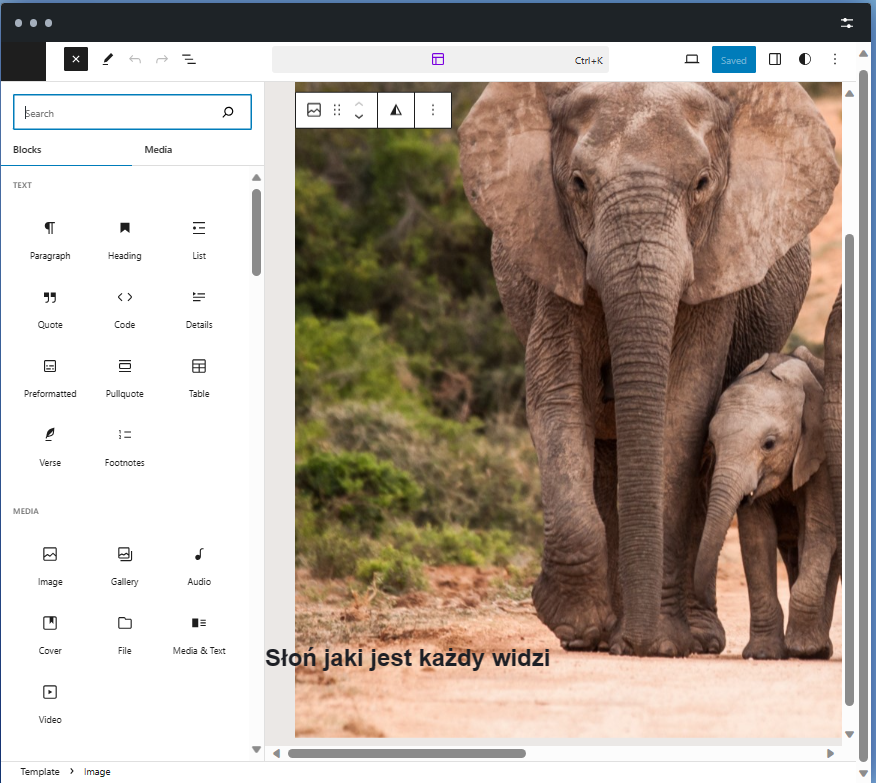
\includegraphics[width=0.8\textwidth]{images/slon_wordpress}
    \captionsource{Wordpress.com}{\cite{WordpressDeveloper2023}}
    \label{fig:wp-plat}
\end{figure}

Rozwój narzędzi do tworzenia stron oraz chęć automatyzacji coraz większej liczby obszarów programistycznych, rozwinął dziedzinę low-code.\ Wśród użytkowników coraz większą popularnością cieszą się platformy low-code \textit{(ang. Low-code Development Platforms, LCDPs)}.\ Takie rozwiązania dostarczają między innymi Google, Microsoft czy Amazon.\ Pozwalają one na tworzenie wysoko skalowalnych rozwiązań przy minimalnym lub zerowym nakładzie pracy z kodem.\ Umożliwia to osobom z niewielkim doświadczeniem w programowaniu, na szybkie wdrożenie oraz tworzenie niezawodnego oprogramowania.\ Twórcy platform oferują również korzystającym, zmniejszenie ilości pracy potrzebnej do wdrożenia albo rozwijania kolejnych funkcjonalności.\ LCDP udostępniane twórcom aplikacji, umożliwiają skalowalność rozwiązań tworzonych na własne potrzeby.\ Dodatkowo są popularne przy tworzeniu aplikacji typu ,,\textit{aplikacja jako usługa}'' \textit{(ang. Software-as-a-Service, SaaS)}, które opłacane są tylko za stopień ich użycia.\ To podejście w konkretnych sytuacjach może się okazać dużo bardziej opłacalne niż utrzymywanie swoich rozwiązań serwerowych.\ Dzięki takim rozwiązaniom wiele małych firm będzie mogło pozwolić sobie na tworzenie i utrzymywanie dostosowanych rozwiązań opartych o ekosystem \textit{Microsoft365} / \textit{Google Workspace}~\cite{Bock2021,Hirzel2022}.


\section{Microsoft PowerApps}
Jest to platforma programistyczna umożliwiająca tworzenie niestandardowych aplikacji dla rozwiązań biznesowych.\ Przykład ekranu platformy przedstawiono na \refsource{rysunku}{fig:pa-plat}.

\begin{figure}[H]
    \centering
    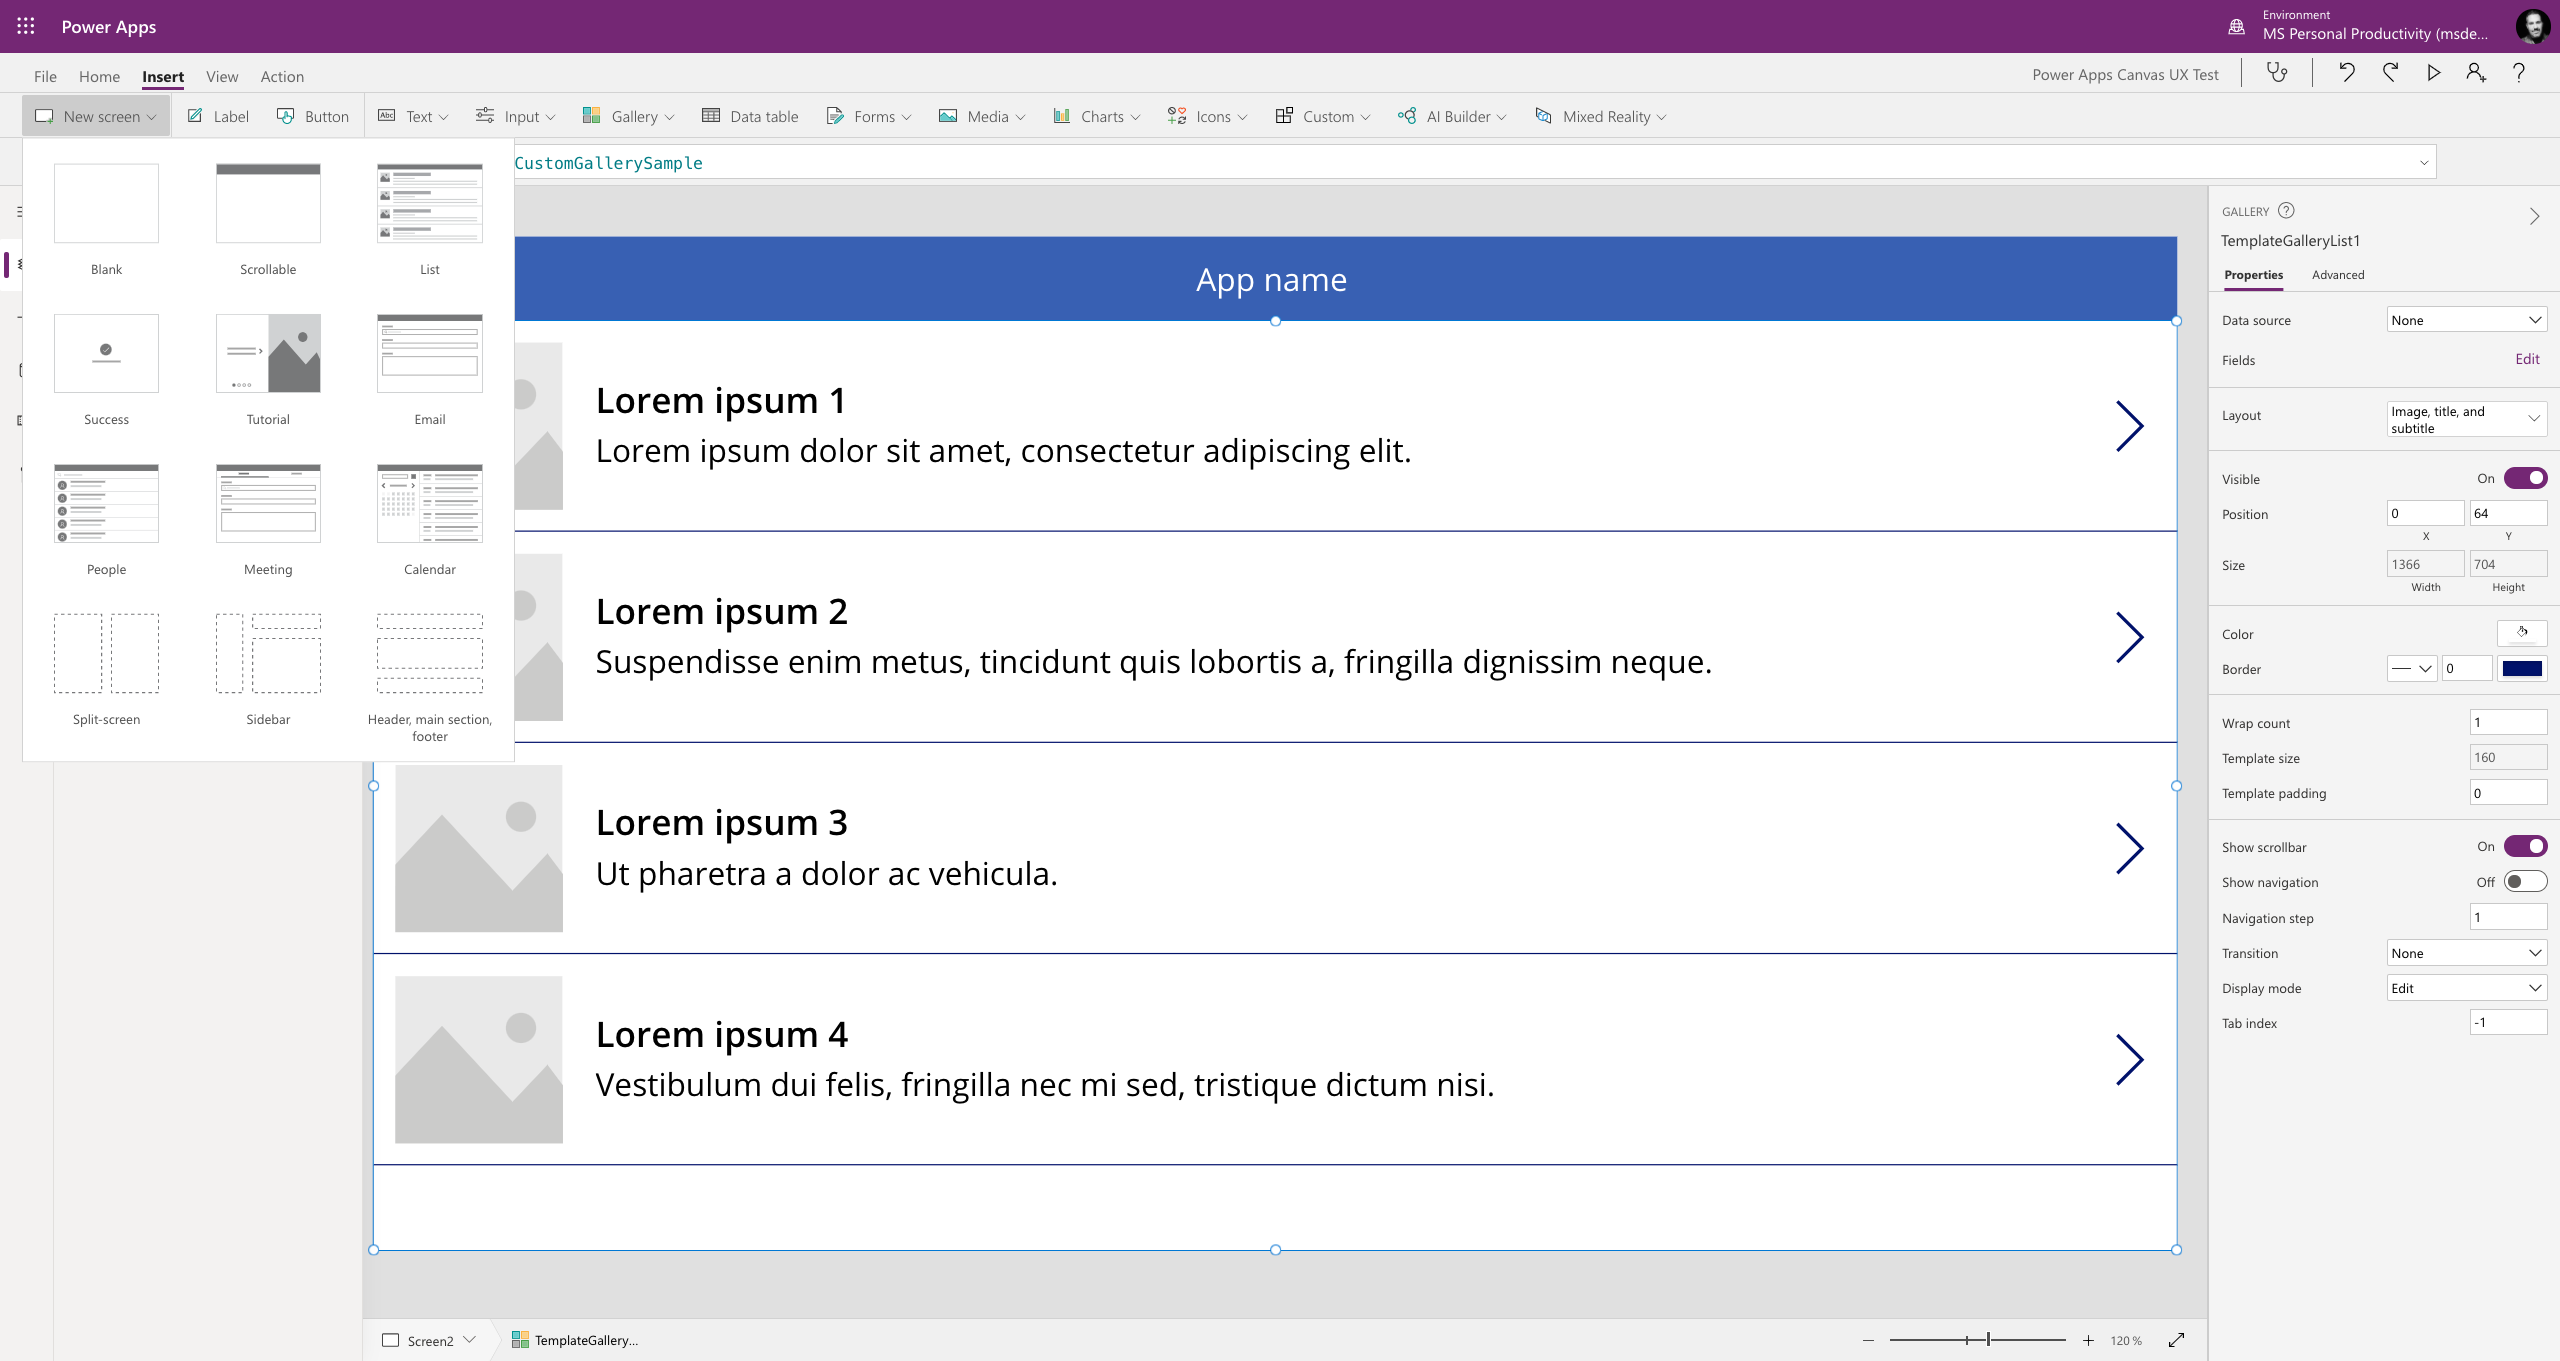
\includegraphics[width=\textwidth]{images/ms_powerapps}
    \captionsource{PowerApps od Microsoft}{\cite{Powerapps2023}}
    \label{fig:pa-plat}
\end{figure}


Microsoft PowerApp umożliwia tworzenie aplikacji opartych o różnorodne źródła danych.\ Do nich należą między innymi: SQL Server, SharePoint, Dynamics 365.\ Zaletą MS PowerApp jest tworzenie aplikacji responsywnych, działających dobrze na wielu rodzajach urządzeń.\ Pozwala też tworzyć trzy typy aplikacji przy braku konieczności kodowania

\begin{itemize}
    \item \textbf{Kanwa} -- typ aplikacji oparty o model danych znajdujący się np. w Excelu.\ Kanwę tworzy się za pomocą przesuwanych kafelek, użytkownik układa je samodzielnie.\ Umożliwia to pełną dowolność w tworzonym interfejsie graficznym.

    \item \textbf{Oparte na modelu} -- aplikacja wygenerowana przy użyciu Microsoft Dataverse.\ Bazuje na modelu danych oraz pozwala na jego analizę.\ Użytkownik może analizować dane, bez znajomości specjalistycznych komend np. z języka Python.

    \item \textbf{Karty} -- aplikacje, które można dodać do usługi Microsoft Teams w określonym biznesowym celu.\ Rozwiązanie to wprowadza możliwość tworzenia aplikacji zespołowo, bez konieczności przełączania się między różnymi platformami.\ Zaletą tego rozwiązania jest możliwość tworzenia małych aplikacji do pojedynczej funkcjonalności~\cite{Microsoft,Microsofta,Microsoftb,Microsoftc}.
\end{itemize}

\section{Amazon QuickSight}
Jest to rozwiązanie firmy Amazon, które umożliwia firmom dostarczanie rozwiązań z zakresu analityki biznesowej \textit{(ang. business intelligence, BI)}.\ Amazon QuickSight udostępnia interaktywne pulpity \textit{(ang. dashboards)}, zawierające narzędzia do analizy danych.\ Użytkownicy mają możliwość korzystania z interaktywnych formularzy, raportów czy zapytań w języku naturalnym.\ Rozwiązanie korzysta z jednego źródła prawdy, określonego przez użytkownika~\cite{AmazonQuickSight}.\ Przykładowy \textit{dashboard} przedstawia \refsource{rysunek}{fig:am-qs}.
\begin{figure}[H]
    \centering
    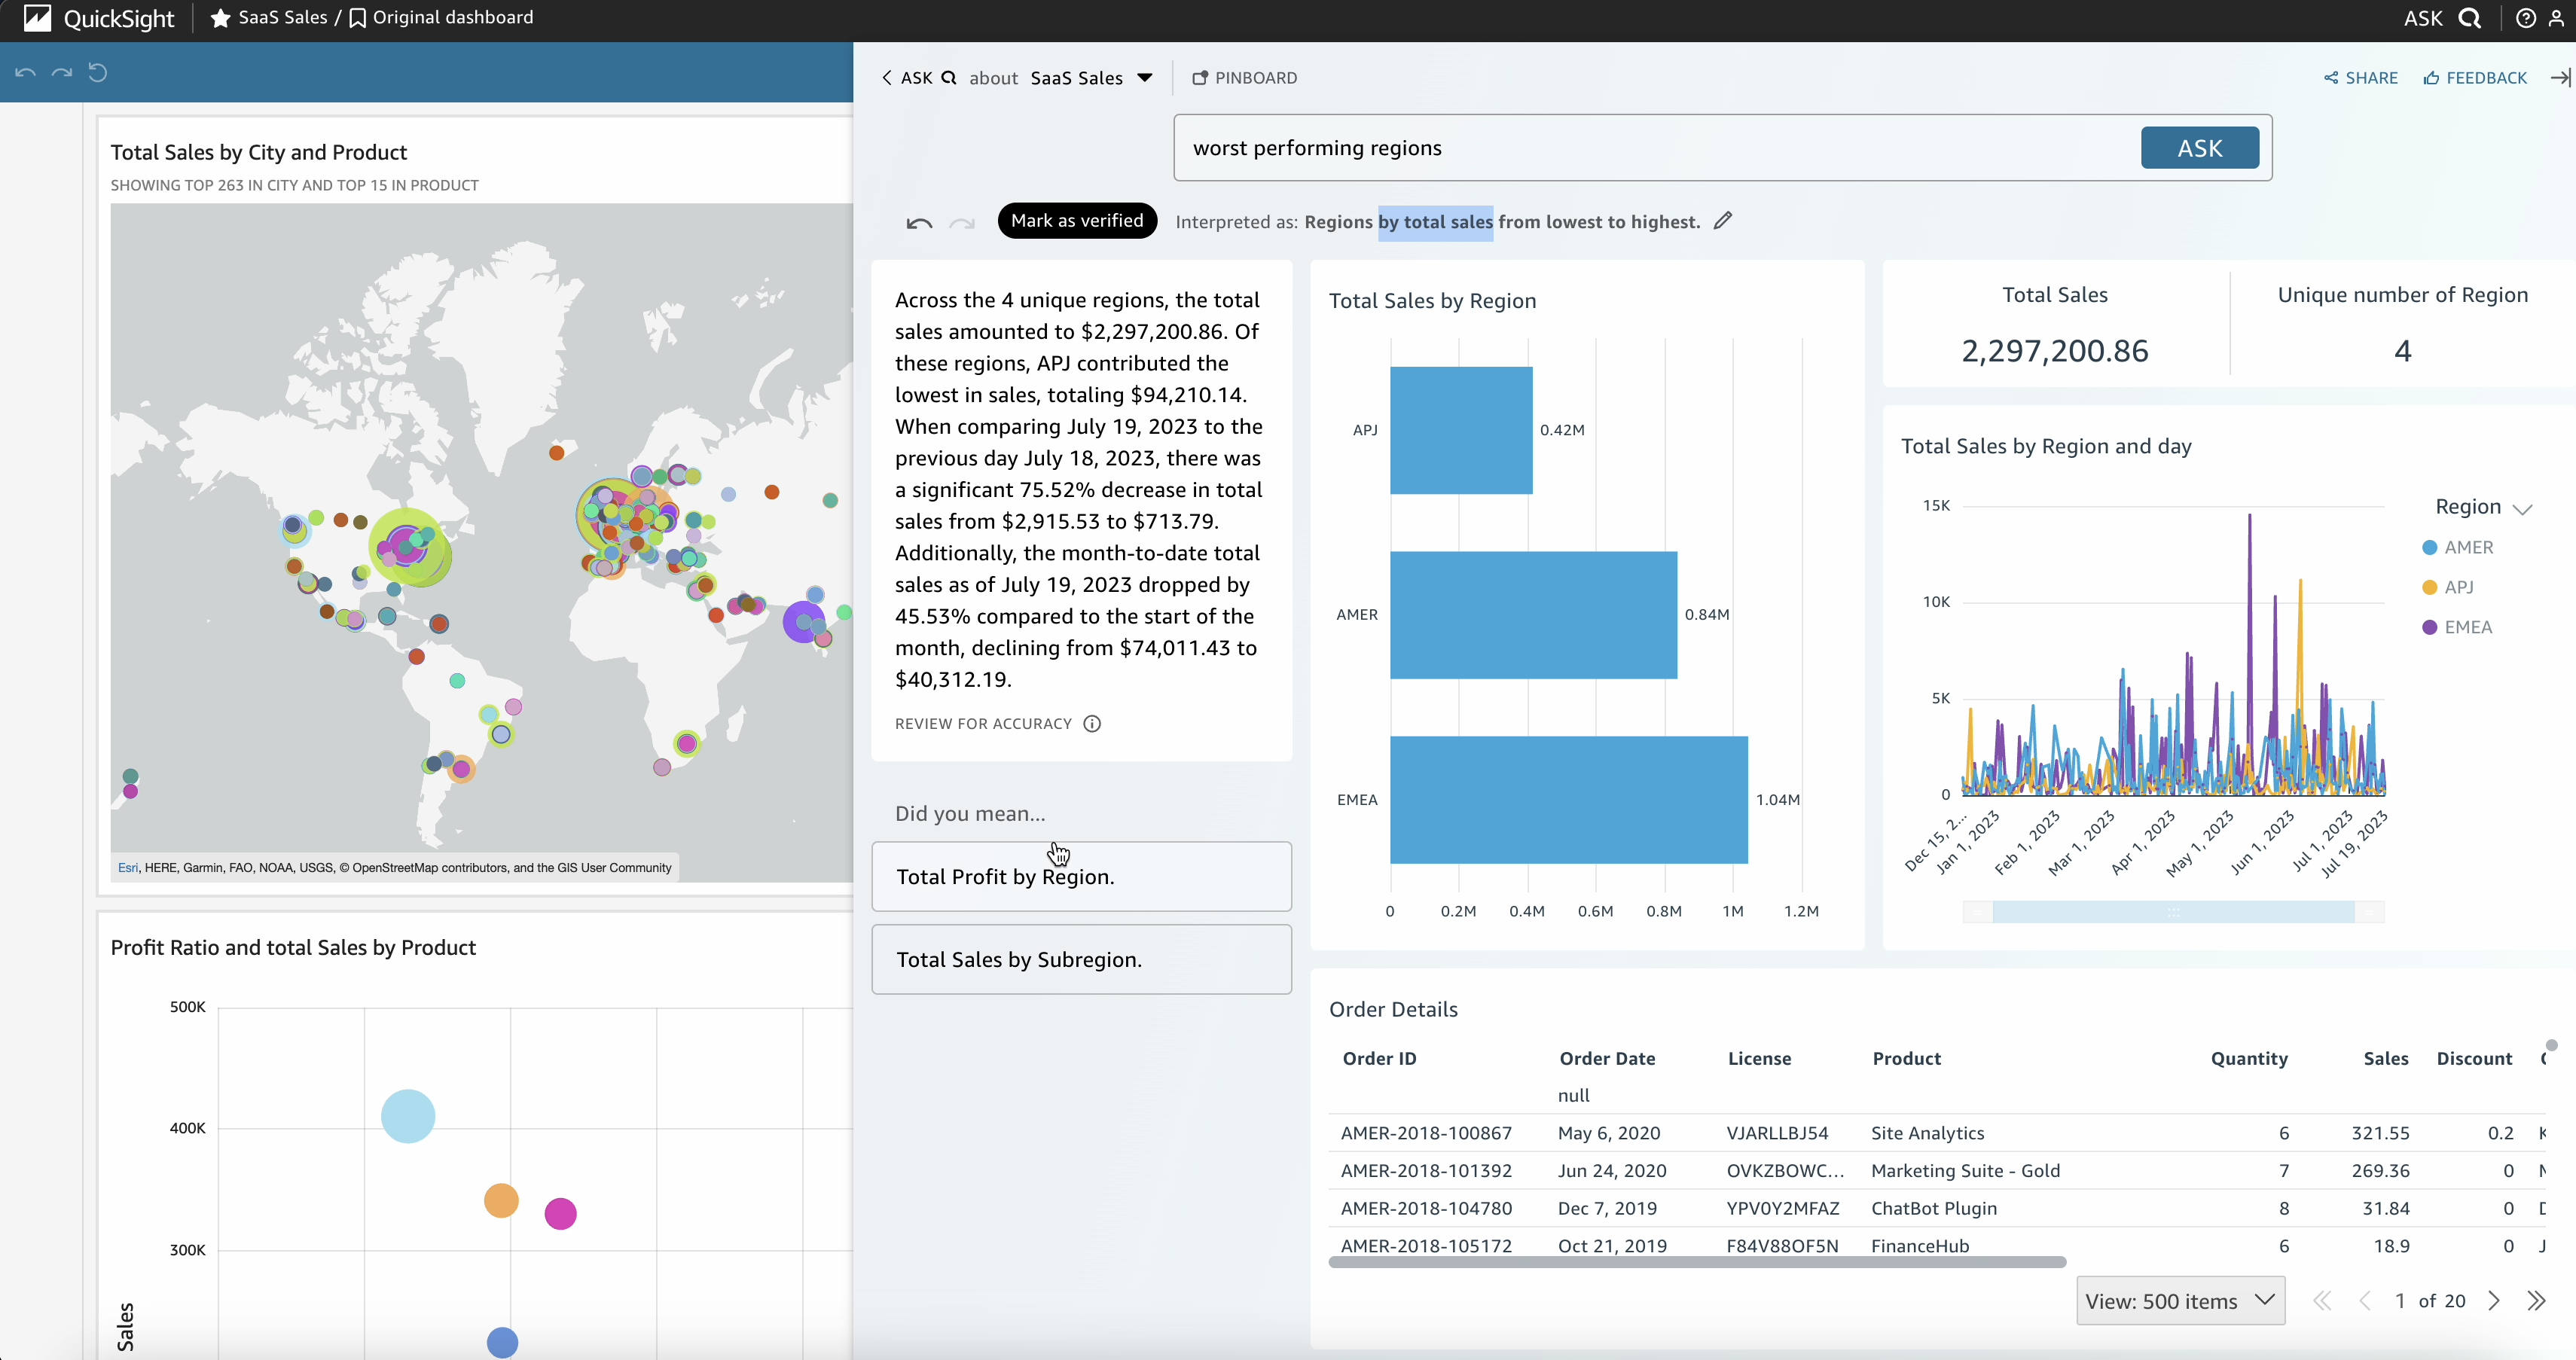
\includegraphics[width=\textwidth]{images/amazon_qs}
    \captionsource{Amazon QuickSight}{\cite{AmazonQuickSight}}
    \label{fig:am-qs}
\end{figure}
\vfill
\clearpage

\section{Google AppSheet}
Platforma AppSheet od firmy Google umożliwia tworzenie aplikacji mobilnych oraz desktopowych bez użycia kodu.\ Firma wskazuje na możliwości integracyjne z różnymi dostawcami danych, do których należą między innymi Microsoft, Dropbox.\ Dodatkowo posiada wbudowaną integrację z aplikacjami Google Workspace, do których należą Gmail, Sheets oraz Spaces.\ Platforma pozwala również na tworzenie automatycznych botów, które wykonują zadania po interakcji z bodźce zewnętrznymi bądź wewnętrznymi.\ Narzędzie pozwala w prosty sposób na tworzenie szybkich rozwiązań biznesowych w ekosystemie firmy Google~\cite{GoogleAppSheet}.\ Przykładowy ekran tworzenia aplikacji prezentuje \refsource{rysunek}{fig:ga-as}
\begin{figure}[H]
    \centering
    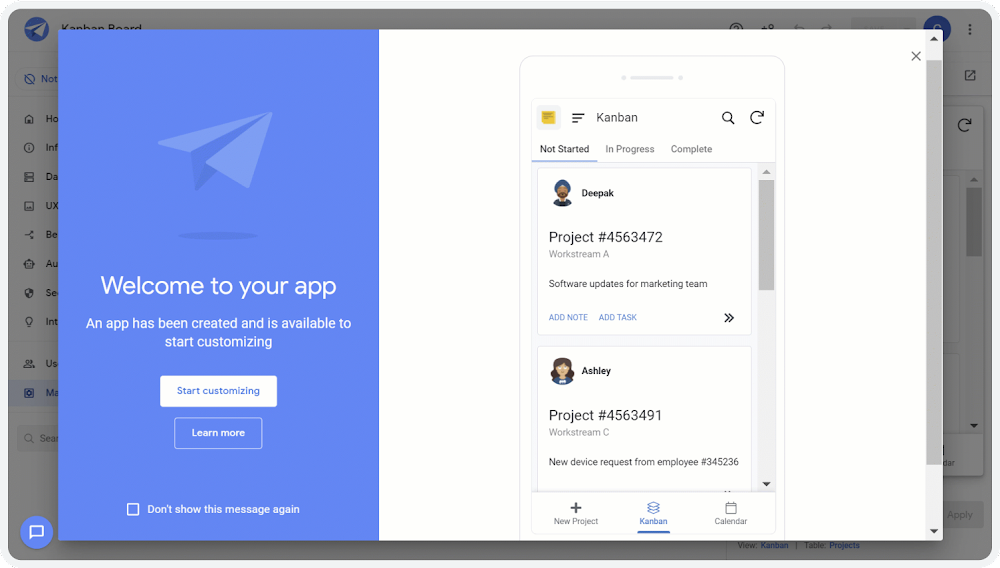
\includegraphics[width=\textwidth]{images/google_as}
    \captionsource{Google AppSheet}{\cite{GoogleAppSheet}}
    \label{fig:ga-as}
\end{figure}